
% Group addresses by affiliation; use superscriptaddress for long
% author lists, or if there are many overlapping affiliations.
% For Phys. Rev. appearance, change preprint to twocolumn.
% Choose pra, prb, prc, prd, pre, prl, prstab, prstper, or rmp for journal
%  Add 'draft' option to mark overfull boxes with black boxes
%  Add 'showpacs' option to make PACS codes appear
%  Add 'showkeys' option to make keywords appear
\documentclass[aps,prl,preprint,groupedaddress]{revtex4-1}
%\documentclass[aps,prl,preprint,superscriptaddress]{revtex4-1}
%\documentclass[aps,prl,reprint,groupedaddress]{revtex4-1}
\usepackage{bm}
\usepackage{amsmath}
\usepackage{graphicx}
\input{papers_packages_command._include_tex}
% You should use BibTeX and apsrev.bst for references
% Choosing a journal automatically selects the correct APS
% BibTeX style file (bst file), so only uncomment the line
% below if necessary.
\bibliographystyle{apsrev4-1}

\begin{document}
\graphicspath{{images/}}

% Use the \preprint command to place your local institutional report
% number in the upper righthand corner of the title page in preprint mode.
% Multiple \preprint commands are allowed.
% Use the 'preprintnumbers' class option to override journal defaults
% to display numbers if necessary
%\preprint{}

%Title of paper
\title{The importance of external priors for the S4 generation of CMB experiments.}

\author{A. Manzotti}
%\email{\href{mailto:manzotti.alessandro@gmail.com}{manzotti.alessandro@gmail.com}}
%\affiliation{Department of Astronomy \& Astrophysics, University of Chicago, Chicago IL 60637}
%\affiliation{Kavli Institute for Cosmological Physics, Enrico Fermi Institute, University of Chicago, Chicago, IL 60637}
\author{S. Dodelson}
%\affiliation{Fermilab Center for Particle Astrophysics, Fermi National Accelerator Laboratory, Batavia, IL 60510-0500}
%\affiliation{Department of Astronomy \& Astrophysics, University of Chicago, Chicago IL 60637}
%\affiliation{Kavli Institute for Cosmological Physics, Enrico Fermi Institute, University of Chicago, Chicago, IL 60637}


\date{\today}

\begin{abstract}
The next generation of CMB experiments is expected to drastically improve our understanding of neutrino physics, inflation, Dark Matter and Dark Energy.
Indeed they will measure with cosmic variance limited precision the temperature and E mode polarization that will also allow the reconstruction of lensing potential with a signal to noise bigger than one on several scales. Detailed forecasts have been done and will tremendously help to plan and motivate the next generation of CMB experiments. However we think that the dependence of this results on the assumed external priors need to be explored. For this reason in this work we use a fisher-matrix technique to test how external priors can lead to improvement in S4 CMB parameters constraint. We find that quite surprisingly CMB S4 are very powerful even on

\begin{itemize}
\item We are now using a simplistic lensing noise but I have lensing noise with the usual Hu Okamoto formula. Iterative Seljack not there yet. Needed?
\item We are varying $\tau, ~ n_{s}, ~ A_{s}, ~ N_{\rm eff}, ~ H_{0}, w,~\Omega_{\nu}h^{2},~\Omega_{c}h^{2},~\Omega_{b}h^{2}$. The neutrino sector consists of one massive neutrino of $m_{\nu}=0.083$ eV, which corresponds to $\Omega_{\nu}h^{2}=0.0009$.
\item Next TODO: Check for bugs and errors code (DONE look at Zhen test). PCA? what prior is more important? Full MCMC should not be extremely hard with cosmosis (I implemented a toy likelihood analysis to be improved).
\end{itemize}


\end{abstract}

% insert suggested PACS numbers in braces on next line
\pacs{}
% insert suggested keywords - APS authors don't need to do this
%\keywords{}

%\maketitle must follow title, authors, abstract, \pacs, and \keywords
\maketitle

% body of paper here - Use proper section commands
% References should be done using the \cite, \ref, and \label commands
\section{Introduction \label{sec:intro}}

Since the first results coming from the COBE experiments great results.

Far from finished S4 experiment will reveal several unclear aspect of the universe like the neutrino sector, Dark Energy and Dark matter properties. 


The number of relativistic species,like neutrinos, present in the early influence alter the expansion history of the universe. This can be probe by CMB by comparing the sound horizon scale with the silk damping. Indeed their ration scales differently with the expansion rate giving $r_{d}/r_{s}\propto\sqrt{H}$ (see \cite{2013arXiv1309.5383A}, \cite{2013PhRvD..87h3008H} and references therein). Their mass on the other hand has very little influence on the CMB physics because for the range of masses allowed by recent constraints neutrinos are relativist at the last scattering surface. As a lot of other low redshift effect however they modify the CMB through the lensing effect of large scale structure on CMB photons. Different neutrino masses led to different growth of structure which consequently lead to different CMB lensing. The lensing potential can be reconstructed from the CMB itself opening the possibilities of constraining the neutrino mass with CMB. In the future according for example to \cite{wu:2014}, CMB alone will constrain $N_{\rm eff}$ with a $1\%$ precision and the total mass of neutrinos at $60\%$ with a consistent factor of two improvement when BAO are added. Even if these constraints depends on the fiducial values used the recent future will be a big step from the neutrino sector.

CMB is also sensitive to Dark energy (see \cite{2010MNRAS.405.2639J}) mainly from its effect on the Hubble function that modifies the distance to the last scattering surface. Furthermore the influence of Dark Energy in the low redshift universe modify the energy of CMB photons through the Integrated sachs wolfe Effect. Also as it was true in the neutrino case, CMB can thorugh lensing probe the growth of structure that depends on the dark energy properties and in particular its equation of state. When trying to constrain dark energy properties however we have to remember that they are strongly degenerate with other geometrical parameters like $H_{0}$ and $\Omega_{k}$. To get competitive constraint, CMB experiments will have to rely on external prior coming from BAO and supernova experiments.

The importance of external priors in the dark energy case lead us to a more general concept. It is certainly true that CMB S4 will open an all new window
but the synergy with other experiments like large scale structure clustering and weak lensing, BAO targeted experiments, SN, and proposed experiments like SPIRE. Indeed forecasted constrains very often assume external realistic prior.

Forecast is important \cite{wu:2014} ... we think that also a detailed study of priors will be important in planning new experiment.

For this reason we...

This paper is organized as follow: in \refsec{method} we in \refsec{results} and we conclude with a discussion of our results in \refsec{conclusions}



\section{Assumption and methods \label{sec:methods} }
We start this section by introducing the Fisher matrix formalism, a simple but powerful technique widely used to forecast future experimental constraints on the parameters of the assumed cosmological model. Then, we describe in details the $\nu\Lambda$CDM cosmological model we use in this work and the fiducial parameters we assume (from recent BAO+CMB). 


\subsection{Fisher Matrix formalism}
The starting point to estimate errors on cosmological parameters is the Bayes theorem that relates the likelihood of measuring a set of data given the parameters of the model ($\mathcal{L}(d|\theta)$) to what we want: the posterior probability of those parameters given the data, $\mathcal{L}(\theta|d)$.
These are related by the prior probability of the parameters $P(\theta)$ through:
\begin{equation}
\mathcal{L}(\theta|d)\propto \mathcal{L}(d|\theta)P(\theta),
\end{equation}
where, as usual, we have neglect the probability of the data itself.
These general framework can be simplified in the context of cosmology by focusing not on the entire posterior distribution but on small perturbations around the maximum of an assumed Gaussian likelihood. 
Indeed we will assume that the likelihood can be approximated as Gaussian.
While this approximate the true likelihood most of the time, the opposite has been found in other cases \cite{2012JCAP...09..009W}. Even if other methods of analysis have been proposed \cite{2006JCAP...10..013P,2006astro.ph..9591A} this is still the standard assumption when future constrains have been forecasted \cite{wu:2014}. Moreover the gaussian approximation gets better at smaller scales which, a part for the exception of the optical depth parameters $\tau$, is where most of the information is coming from in our case.
Secondly we will assume to know the true ``fiducial'' parameters that maximize the likelihood $\mathcal{L}(\theta|d)$. Given that we are then able to estimate the uncertainties on those parameters by a simple analysis of the likelihood curvature around the fiducial values.
As usual we define the fisher matrix elements as:
\begin{equation}
	\centering
		F_{ij} \equiv - \left\langle\frac{\partial^2 \log \mathcal{L}}{\partial \theta_i \partial \theta_j} \bigg|_{\boldsymbol{\theta} = \boldsymbol{\theta_0}}\right\rangle,
	\label{eq:Fij_def}
\end{equation}
where $\theta_{i,j}$ represents two of the parameters and $\boldsymbol{\theta_0}$ is the parameters array that, by definition, maximize the likelihood.
We refer the reader to \cite{} for a detailed explanation of the fact that with the usual definition of power spectrum $<a_{\ell m}^{X}a_{\ell' m'}^{Y}>=\delta_{\ell \ell'}\delta_{mm'}C^{X,Y}$ with $X,Y\in\{T,E,\phi\}$ the Fisher matrix can be rewritten as:
\begin{equation}
 F_{ij} = \sum_\ell \frac{2\ell+1}{2} f_{sky} {\rm Tr} \left(  \boldsymbol{C}^{-1}_\ell( \theta) \frac{\partial \boldsymbol{C}_\ell}{\partial \theta_i} \boldsymbol{C}^{-1}_\ell( \theta) \frac{\partial \boldsymbol{C}_\ell}{\partial \theta_j}  \right)
 \end{equation}
 with $\boldsymbol{C}_\ell$ encapsulating the usual power spectra in a matrix structure:
 \begin{eqnarray}
 	\centering
		\mathbf{C}_\ell \equiv \left( \begin{array}{ccc}C_\ell^{TT} + N_\ell^{TT} & C_\ell^{TE} & C_\ell^{Td} \\ C_\ell^{TE} & C_\ell^{EE} + N_\ell^{EE} & 0 \\ C_\ell^{Td} & 0 & C_\ell^{dd} + N_\ell^{dd}\end{array}\right).
	\label{eq:cov_definition}
\end{eqnarray}
The terms $N_\ell^{X}$ represents the instrumental noise of the experiment and will be discussed in \refsec{noise}.
The power of this method descend from Cramer-Rao inequality that relates the errors on parameter $i$ marginalized over all the other parameters $\sigma_i$ to the Fisher matrix as:
\begin{equation}
\sigma_i \equiv \sigma (\theta_i) = \sqrt{(\mathbf{ F^{-1}})_{ii}}.
\label{eqn:cramer-rao}
\end{equation}

This powerful and simple approach however introduce some technical difficulties together with the previously mentioned assumption that the likelihood is gaussian. Indeed it is known that increasing the number of parameters used in the analysis can lead to numerical issues. Fisher matrix  can become ill-conditioned: a small change in the fisher matrix led to a big change in its inverse. Given \refeq{cramer-rao} this can be a problem for error estimation. While we understand this as possible concern we carefully compare our results to the literature  \footnote{we thank the authors of \cite{pan:2015} for their collaboration.}
Furthermore we use the same technique used in \cite{2006astro.ph..9591A} to avoid possible numerical instability in the marginalizing procedure. This allow not to invert the entire matrix when we want to marginalize over a set of parameters minimizing numerical issue and conserving parameters degeneracies as much as possible.

Priors on cosmological parameters coming from external experiments, the main focus or our work can be easily treated in this contest.
For example a $1\%$ prior on $H_{0}$ can be obtained by:
\begin{equation}
F_{H_0 H_0} \rightarrow F_{H_0 H_0} + \frac{1}{(1\% \times H_{0,\text{fid}})^2}, 
\end{equation}



\begin{figure}[htbp]
\begin{center}
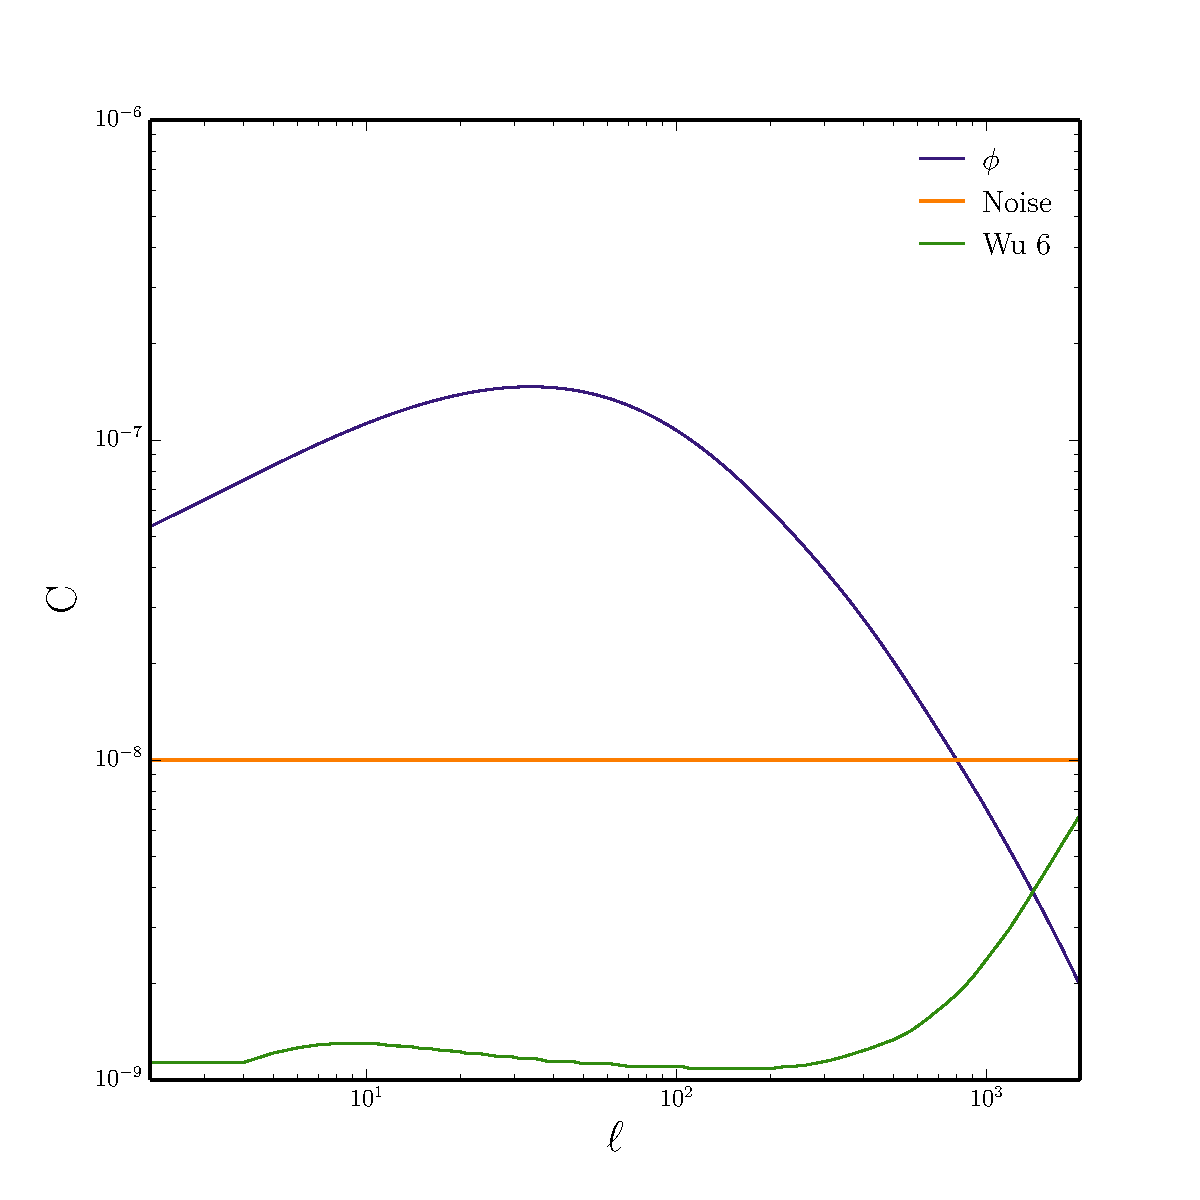
\includegraphics[scale=0.6]{PS_phi_with_noise.pdf}
\caption{Lensing potential power spectrum for our fiducial cosmology together with the lensing reconstruction noise $N^{\phi}$ used in this work.}
\label{fig:phi-cl-noise}
\end{center}
\end{figure}

\begin{figure}[htbp]
\begin{center}
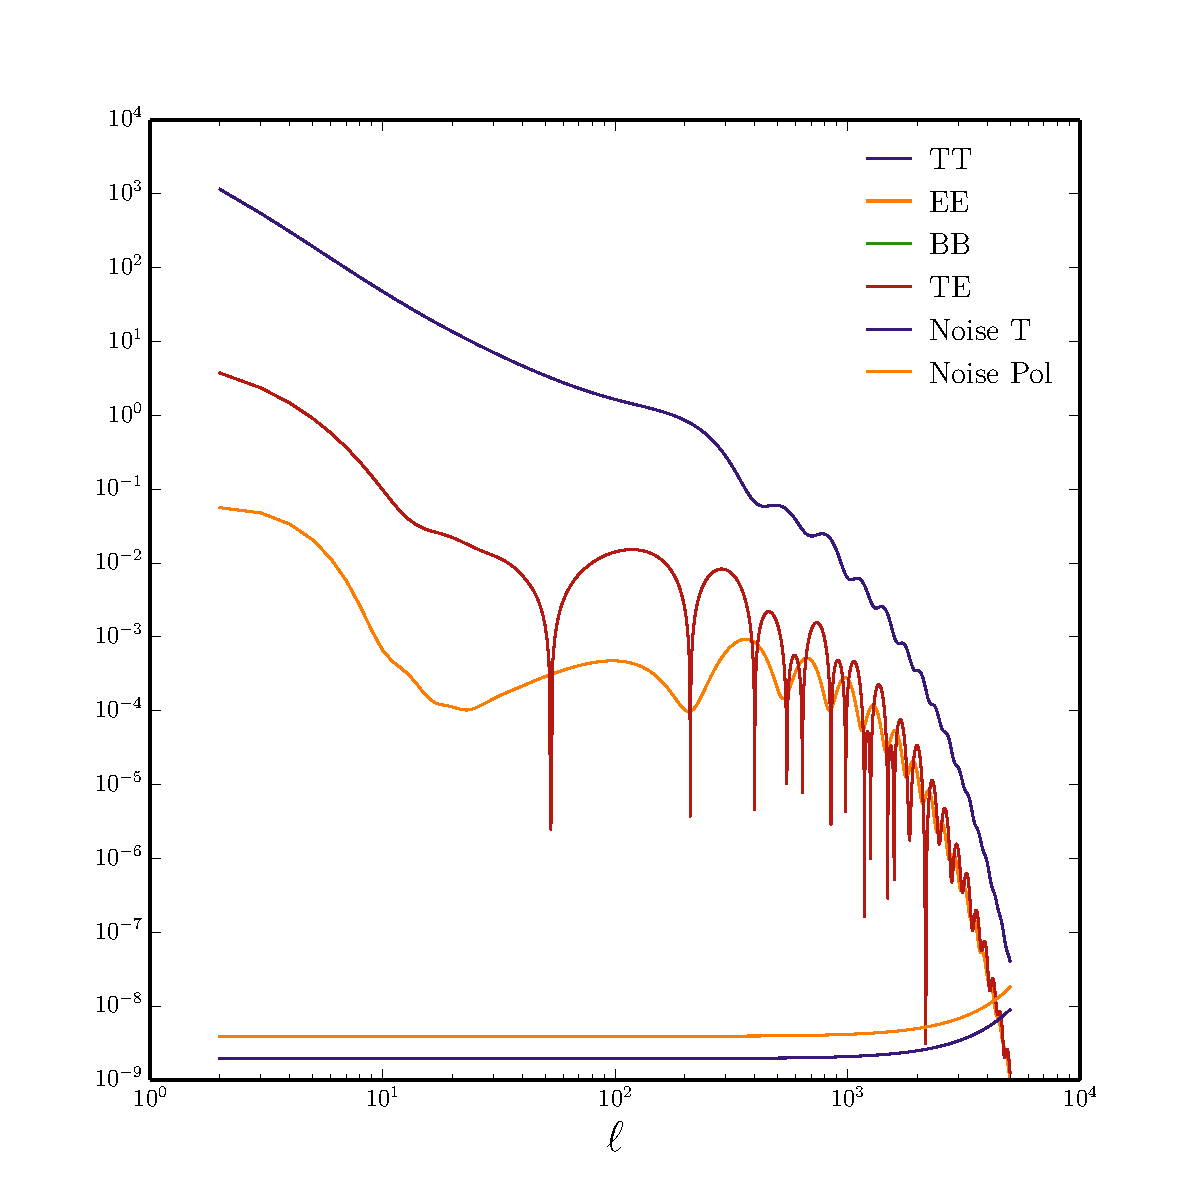
\includegraphics[scale=0.6]{PS_with_noise.pdf}
\caption{CMB power spectrum for our fiducial cosmology together with the instrumental noise used in this work. They are basically equivalent to a cosmic variance limited experiment with $l_{max}\sim 3000$}
\label{fig:cmb-cl-noise}
\end{center}
\end{figure}


\subsection{CMB S4 experiments: level of noise.\label{sec:noise}}

The next generation of CMB experiments defined as S4 will have an extraordinary resolution and depth.\
We will also assume that for the measurement we use, the temperature and E-mode polarization of the CMB large scale foreground like dust are under control and negligible. We will deal with the poisson noise in the temperature signal by discarding all the small scales modes with $\ell>\ell_{T,max}=3000$.
The remaining source of noise, the instrumental noise is added to the power spectrum in the usual way:
 \begin{equation}
 	\centering
		N^{ XX' }_\ell = s^{\, 2} \exp \left(\ell(\ell+1) \frac{\theta^{\ 2}_{\textsc{fwhm}}}{8\log2}\right),
	\label{eq:beamnoise}
\end{equation}
where $\theta^{\ 2}_{\textsc{fwhm}}$ is the FWHM of the experiment's beam and $s$ represent instrumental the white noise.
We decide to use a $1.5$ muK and a beam of 1 arcmin.
Note that  $s \rightarrow s\times \sqrt{2}$ in the case of $ XX' = \{ EE, BB \}$.


Together with E and T we will also consider the information contained in the  
lensing potential $phi$ reconstructed from CMB experiments. The lensing potential represents the integration along the line of site of the gravitational potential and it leaves its signature in the CMB, both in temperature and polarization, by bending CMB photons. This introduce non gaussianities that couples different modes in the otherwise independent CMB modes and using a quadrature estimator technique it can be reconstructed \cite{okamoto:2003,hu:2002}.
For the noise associated to the recosntructed $\phi$ we follow \cite{okamoto:2003,hu:2002} without using more advanced iterative techniques.

We parametrize our cosmology using a flat $\nu \Lambda$CDM universe. We also allow different Dark Energy framework by introducing the equations of state parameter w as a free parameter.

We use the $\Lambda$CDM parameter values from Table 2 of \textit{Planck} best fit value \cite{planck-collaboration:2014g}, i.e. $\Omega_c h^2 =  0.12029$,  $\Omega_b h^2  = 0.022068$, $A_s = 2.215\times10^{-9}$ at $k_0 = 0.05\ {\rm Mpc}^{-1}$, $n_s = 0.9624$, $\tau = 0.0925$, and $H_0 = 67.11$ km/s/Mpc. Regarding the $\Lambda$CDM extension we chose a neutrino energy densities$\Omega_{\nu} h^2$=0.0009, which corresponds to $M_{\nu}$  $\simeq$ 85\ meV and we also set $w=1$.


%\begin{eqnarray}
%\centering
%	s\ [\;\mu {\rm K.arcmin}\;] \equiv \frac{ {\rm NET}\ [\; \mu{\rm K.}\sqrt{s}\;] \times \sqrt{f_{sky} \ [\;{\rm arcmin}^2\;] }}{ \sqrt {N_{\rm det} \times Y \times \Delta T\ [\;{\rm s }\;]}}.
%	\label{eq:sensitivity_definition}
%\end{eqnarray}
%



%\begin{eqnarray}
%	T_{\nu} = \left( \frac{4}{11} \right)^{1/3} T_{\gamma} 
%	\label{eq:tnu_propto_tgamma}
%\end{eqnarray}

\section{Results: \label{sec:results}}

\begin{table}[htdp]
\caption{Fiducial values used.}
\begin{center}
\begin{tabular}{|c|c|}
\hline
$H_{0}$ &\\
\hline
\hline
$\tau$ &  \\
\hline

\hline
$A_{s}$ & \\
\hline

\hline
$n_{s}$ & \\
\hline

\hline
$N_{eff}$ & \\
\hline
\end{tabular}
\end{center}
\label{default}
\end{table}%

\begin{table}[htdp]
\caption{How well we do constrain separate parameters with this data without any external prior?}
\begin{center}
\begin{tabular}{|c|c|c|c|c|c|c|}
\hline
$H_{0}$ &$ M_{\nu}$ &$\Omega_{bc}h^{2}$&$\Omega_{b}h^{2}$&$\tau$&$A_{s}$&$n_{s}$ \\
$0.80 \%$&$40.92\%$&$0.44\%$&$0.11\%$&$3.075\%$&$0.53\%$&$0.18\%$\\

\hline


\end{tabular}
\end{center}
\label{default}
\caption{Things to notice: this is done with the Zhen test parameters ($\ell<3000$ and no error on lensing). Now if we trust it CMB alone can get a $0.8\%$ error on $H_{0}$ thus I am not surprised if a prior on H would not help. However what do we think about it? is it really CMB better than SN. People will not agree on that. $\tau$ will probably improve and also M$\nu$ from BAO may help improving parameters.}
\end{table}%


%\begin{figure}[htbp]
%\begin{center}
%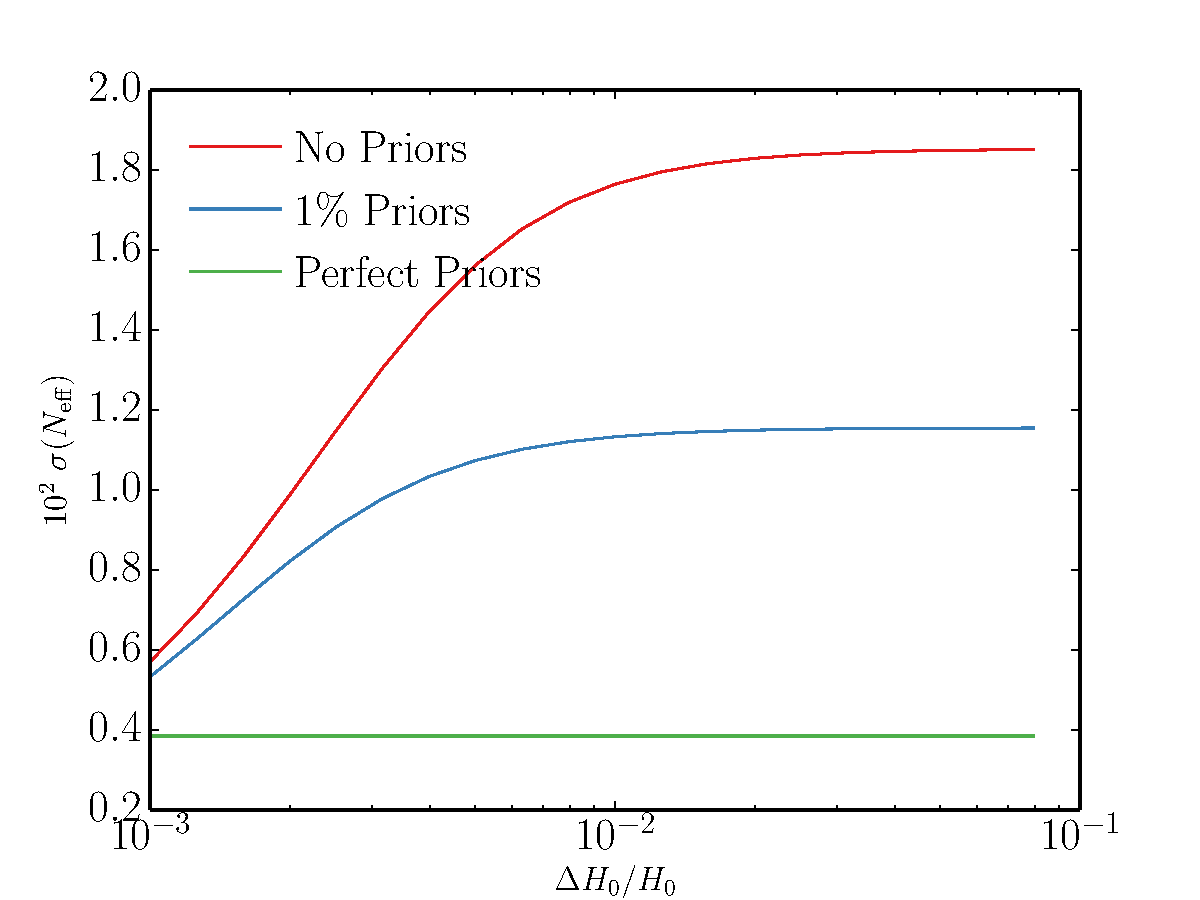
\includegraphics[scale=0.6]{h0_fisher.pdf}
%\caption{}
%\label{fig:phi-cl-noise}
%\end{center}
%\end{figure}
%
%\begin{figure}[htbp]
%\begin{center}
%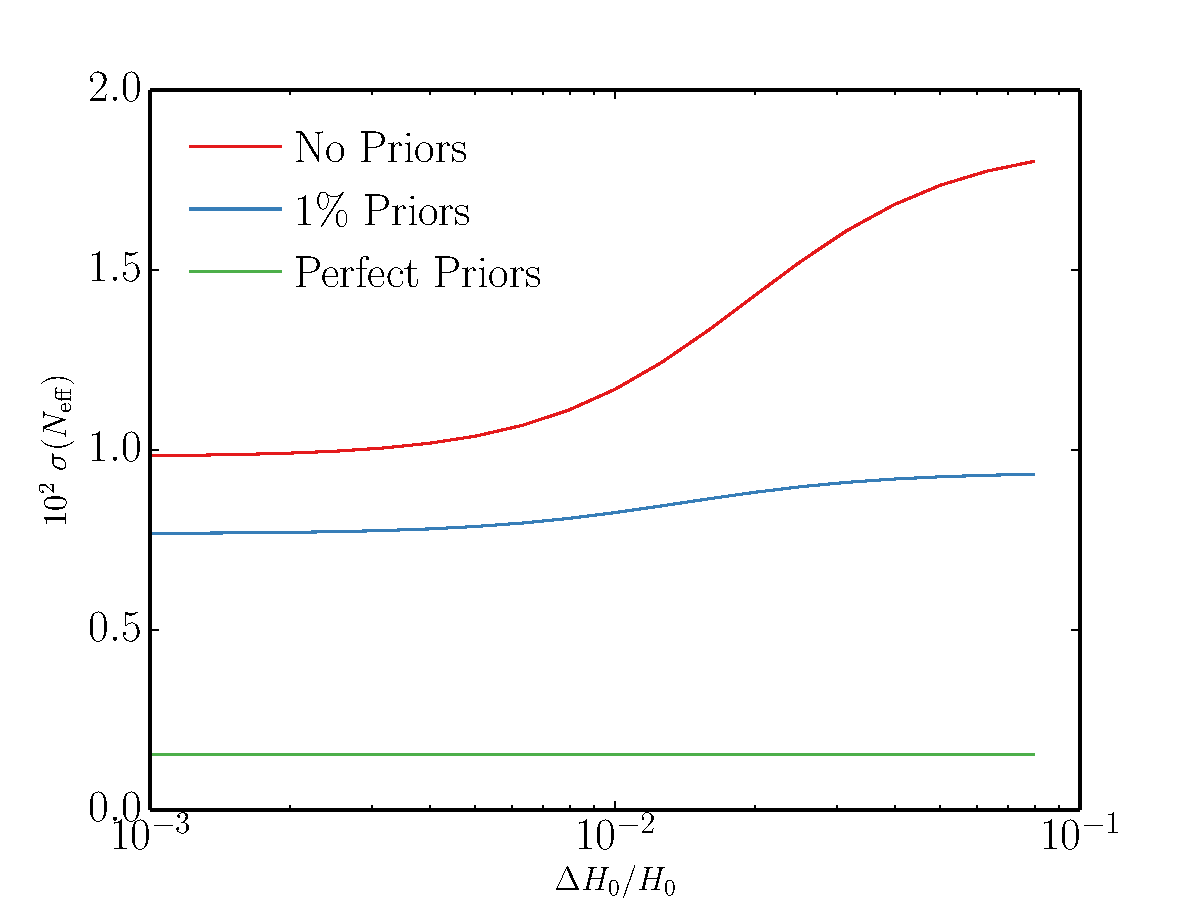
\includegraphics[scale=0.6]{tau_fisher.pdf}
%\caption{}
%\label{fig:phi-cl-noise}
%\end{center}
%\end{figure}



\section{Conclusions \label{sec:conclusions}}
We find that...

This means that supernova experiments CMB spatial distortions and large scale structure can/will/should

Future works

% If in two-column mode, this environment will change to single-column
% format so that long equations can be displayed. Use
% sparingly.
%\begin{widetext}
% put long equation here
%\end{widetext}

% figures should be put into the text as floats.
% Use the graphics or graphicx packages (distributed with LaTeX2e)
% and the \includegraphics macro defined in those packages.
% See the LaTeX Graphics Companion by Michel Goosens, Sebastian Rahtz,
% and Frank Mittelbach for instance.
%
% Here is an example of the general form of a figure:
% Fill in the caption in the braces of the \caption{} command. Put the label
% that you will use with \ref{} command in the braces of the \label{} command.
% Use the figure* environment if the figure should span across the
% entire page. There is no need to do explicit centering.

% \begin{figure}
% \includegraphics{}%
% \caption{\label{}}
% \end{figure}

% Surround figure environment with turnpage environment for landscape
% figure
% \begin{turnpage}
% \begin{figure}
% \includegraphics{}%
% \caption{\label{}}
% \end{figure}
% \end{turnpage}

% tables should appear as floats within the text
%
% Here is an example of the general form of a table:
% Fill in the caption in the braces of the \caption{} command. Put the label
% that you will use with \ref{} command in the braces of the \label{} command.
% Insert the column specifiers (l, r, c, d, etc.) in the empty braces of the
% \begin{tabular}{} command.
% The ruledtabular enviroment adds doubled rules to table and sets a
% reasonable default table settings.
% Use the table* environment to get a full-width table in two-column
% Add \usepackage{longtable} and the longtable (or longtable*}
% environment for nicely formatted long tables. Or use the the [H]
% placement option to break a long table (with less control than 
% in longtable).
% \begin{table}%[H] add [H] placement to break table across pages
% \caption{\label{}}
% \begin{ruledtabular}
% \begin{tabular}{}
% Lines of table here ending with \\
% \end{tabular}
% \end{ruledtabular}
% \end{table}

% Surround table environment with turnpage environment for landscape
% table
% \begin{turnpage}
% \begin{table}
% \caption{\label{}}
% \begin{ruledtabular}
% \begin{tabular}{}
% \end{tabular}
% \end{ruledtabular}
% \end{table}
% \end{turnpage}

% Specify following sections are appendices. Use \appendix* if there
% only one appendix.
\appendix
\section{Appendix I}
\begin{equation}
G = F^{\phi\phi} - F^{\phi\psi}U\Lambda^{-1}U^{T}F^{\phi\psi},
\end{equation}
where we define $\phi = \{N_{eff},...\}$ and $\psi = \{\Omega_{m} ... marginal\}$; therefore, $F^{\phi\phi}$ is the block of the total Fisher matrix containing the parameters we want to constrain, whilst $F^{\psi\psi}$ is the nuisance-parameter Fisher sub-matrix. Here, $\Lambda$ is the diagonal matrix whose elements are the eigenvalues of $F^{\psi\psi}$, whilst U is the orthogonal matrix diagonalising $F^{\psi\psi}$. By using Eq., our marginalizing procedure is more stable, since degeneracies in $F^{\phi\phi}$ are properly propagated to G with no instabilities, and we do not even worry about a possibly ill-conditioned $F^{\phi\phi}$ sub-matrix, since we check its stability on the fly by the diagonalisation.

%\section{}

\begin{acknowledgments}
We thank Youngsoo Park for his contribution in the early stage of this work.
AM want to thank Zhen Pan who allow a careful comparison of our results.
This work was partially supported by the Kavli Institute for Cosmological Physics at the University of Chicago through grants NSF PHY-1125897 and an endowment from the Kavli Foundation and its founder Fred Kavli.
%%%=================================================================
The work of SD is supported by the U.S. Department of Energy, including grant DE-FG02-95ER40896.
\end{acknowledgments}

% Create the reference section using BibTeX:
\bibliography{N_eff_prior_paper}

\end{document}




%
% ****** End of file apstemplate.tex ******

